\chapter{InstaGame}\label{chap:method}


InstaGame is an innovative platform designed to empower educators by enabling the creation of customizable educational games. Building on existing research, InstaGame addresses key limitations found in similar tools, such as SGAME \cite{sgame2020}. While SGAME integrates SCORM-compliant learning objects into preexisting games, it restricts game creation to predefined templates and educational fields, limiting flexibility and broader applicability. Additionally, SGAME's language support is limited to Spanish, narrowing its accessibility for global users. InstaGame overcomes these challenges by offering a more versatile and inclusive solution that accommodates diverse educational needs, linguistic preferences, and content areas.

The work presented enables instructors to tailor games to diverse educational contexts by adapting templates to align with various curricula. Each game template excels in specific fields due to its unique mechanics and design, allowing educators to select the most suitable option for their goals. InstaGame further emphasizes user-friendly tools, making it accessible to educators with varying technical expertise, thereby fostering an engaging and inclusive learning environment. InstaGame also alllows the instructor to create games from any device with an internet browser, ensuring that educators can easily integrate the platform into their teaching practices without the need to install additional software or learn complex programming languages and game design. Once the instructor generates a game, they can share it with students through multiple channels, including unique links, QR codes, and game codes, ensuring broad accessibility and seamless distribution.

\section{Design and Architecture}

The architecture of InstaGame is designed to provide seamless accessibility and scalability. Leveraging a web-based framework, the platform ensures that instructors and students can access the tool from any device with an internet browser. Figure \ref{fig:architecture} illustrates the system’s architecture, which integrates a robust cloud-based backend to manage and store game data.

The instructor portal is built using Next.js, a React framework known for its server-side rendering capabilities and efficient performance. Firebase, a Backend as a Service (BaaS) platform, is employed for real-time database management, ensuring that game data is stored and can be accessed from anywhere. A cloud storage is also used to store game assets, such as images, and Appwrite, open-source service, was adopted for storage solutions. The architecture prioritizes reliability and accessibility to support educators in generating and sharing educational games.

\begin{figure}
	\centering
	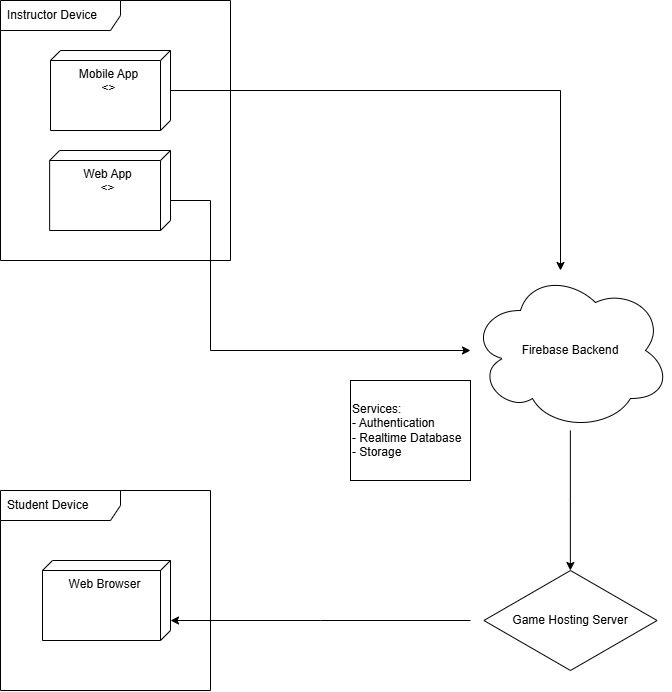
\includegraphics[width=0.8\textwidth]{figures/Deployment_UML.jpg}
	\caption{System Architecture}
	\label{fig:architecture}
\end{figure}

\section{Game Customization System}

InstaGame’s customization system is designed to provide instructors with the tools they need to tailor educational content to their specific requirements. The platform supports the creation of games that encompass a wide range of educational fields and contexts, enabling instructors to design experiences that align with their teaching objectives.

For instance, the click-based puzzle game template allows instructors to upload images, define clickable regions, and input corresponding educational content such as dialogues, questions, and explanations, as shown in Figure \ref{fig:customizationClickPuzzle}. The system’s user-friendly interface ensures that instructors can easily navigate and input data. Additionally, the platform supports the creation of multiple levels, each with distinct content and objectives, enabling instructors to design comprehensive games that cater to diverse learning needs. This versatility accommodates study fields ranging from anatomy and geography to engineering and history.

\begin{figure}
	\centering
	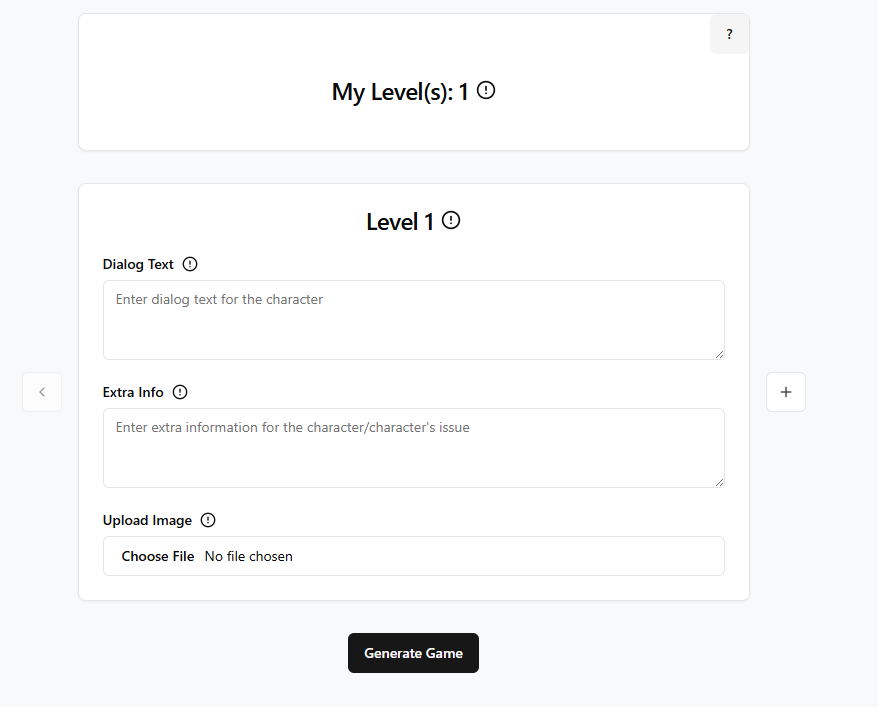
\includegraphics[width=0.8\textwidth]{figures/Diagnose_Game/Instructor_Portal_Diagnose_Game.png}
	\caption{Game Customization System for Click-based Puzzle Game}
	\label{fig:customizationClickPuzzle}
\end{figure}


Another game template, the Space Invaders-like game, enables instructors to input questions and choices, which are displayed as enemies. Players must answer questions correctly by eliminating the enemies holding the correct answers. Instructors can customize various elements, including the title text displayed at the top of the screen, whether the game requires players to convert a goal into an answer (conversion game), the characters displayed on enemies (representing the choices), the possible goals that the system can choose from, and the number of turns within the level. Notably, the number of turns must be odd to determine if the player has won or lost the level, this is calculated by the system based on the majority of correect turns that have been won, for example, if the level has 5 turns, the player must win 3 turns to win the level, or if the level has 7 turns, the player must win 4 turns to win the level.

\begin{figure}
	\centering
	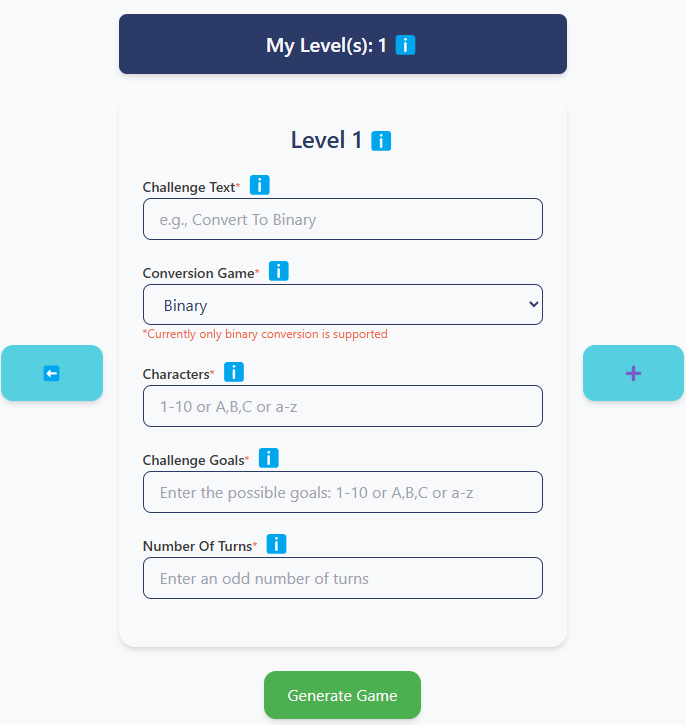
\includegraphics[width=0.8\textwidth]{figures/Space_Invaders/Instructor_Portal_Space_Invader.png}
	\caption{Game Customization System for Space Invaders-like Game}
	\label{fig:customizationSpaceInvaders}
\end{figure}

Both templates adhere to the MDA \cite{MDA2004} game design framework, which consists of mechanics, dynamics, and aesthetics. The mechanics are the rules and procedures that guide the player's actions, such as answering questions or clicking on images. The dynamics refer to the interactions between the player and the game, such as the feedback provided after answering a question. The aesthetics are the emotional responses elicited by the game, such as the sense of accomplishment when completing a level.

In addition to the MDA framework, the templates also align with the elemental pentad framework, which is a more comprehensive approach directed toward game-based learning (GBL). The elemental pentad, which is another framework derived from the more famous elemental tetrad \cite{tetrad2011}, consists of five elements: mechanics, story, aesthetics, technology, and pedagogy \cite{ahmad2019}. The mechanics refer to the rules and procedures that guide the player's actions, such as answering questions or clicking on images, as mentioned earlier. The story represents the narrative that contextualizes the game, such as the dialogue present in the click-based puzzle game. The aesthetics refer to the emotional responses evoked by the game \cite{MDA2004}, such as the sense of accomplishment upon completing a level, as previously noted. The technology refers to the platform used to deliver the game, such as a web browser or mobile device. The pedagogy pertains to the educational theories that inform the game design, such as constructivism or behaviorism.

By incorporating these elements, the templates provide a comprehensive learning experience that engages students while supporting educational goals. Notably, these elements are always present but are slightly altered based on the instructor's input. For example, the mechanics are determined by the instructor's questions and choices, the story is influenced by the instructor's dialogue and explanations, the aesthetics are shaped by the instructor's feedback and rewards, the technology is determined by the platform used to access the game, and the pedagogy is informed by the instructor's educational objectives.



\section{Game Sharing System}

InstaGame features a streamlined game sharing system designed to facilitate easy distribution of educational games to students. Once a game is generated, the platform generates a unique link (view game button in \ref{fig:shareGame}), a QR code, and a game code, as shown in \ref{fig:shareGame}. 
\begin{figure}
	\centering
	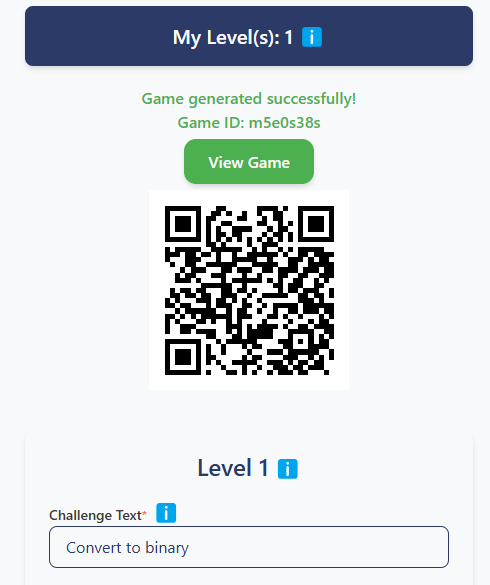
\includegraphics[width=0.8\textwidth]{figures/Space_Invaders/Instructor_Portal_Space_Invader_Generated_Links.jpeg}
	\caption{Game Sharing System}
	\label{fig:shareGame}
\end{figure}
These sharing options provide instructors with multiple ways to distribute the game, catering to various classroom setups and technological capabilities.

The generated link can be shared directly via email or messaging platforms, while the QR code allows students to access the game instantly using their devices. The game code serves as an additional access method, particularly useful in scenarios where students are using a shared portal or platform to enter their assigned activities. This multi-faceted sharing system ensures flexibility and convenience, enabling broad accessibility for both instructors and students. This ensures that the instructor can share the game with the students in a way that is most convenient for them, saving time and effort in the process, and incase the instructor wants save the game for future use, the game code can be used to access the game at a later time, by saving the game link or qr code, the instructor can easily access the game at a later time, without the need to generate a new game, this is particularly useful for games that are used frequently or for multiple classes.


% TODO show game screenshots
\section{Gameplay}

InstaGame supports two game templates, a Space Invaders-like game and a click-based puzzle game, each offering unique gameplay mechanics tailored to different learning objectives.

In the Space Invaders-like game, players engage in fast-paced gameplay where they must eliminate enemies before they reach the bottom of the screen or hit the player with a projectile. This template is well-suited for reinforcing quick decision-making and recall in subjects like mathematics or vocabulary. The click-based puzzle game, on the other hand, offers a more relaxed experience, requiring players to solve puzzles by identifying correct answers within an image. For example, an anatomy-based game could task players with diagnosing a condition by selecting the appropriate organ.

\section{Goal Checking System}
The goal checking system ensures that player actions are evaluated against predefined criteria set by the instructor. This allows for accurate assessment of student performance and ensures that gameplay aligns with educational objectives. By integrating these systems, InstaGame fosters a balance between engaging gameplay and meaningful learning outcomes. This ensures that the instructor has full control over what is considered a correct answer, and the student has control over their answer, and as a foundational concept of the platfrom, the students input is compared to the instructors input to determine if the answer is correct or not. In pseudocode, the goal checking system would look like the following:
\begin{verbatim}
	1. Initialize Goal Checking System:
	   - Define `correctAnswer` as the input provided by the instructor.
	   - Define `studentInput` as the answer submitted by the student.
	
	2. Receive Student Input:
	   - Prompt the student to submit their input.
	   - Store the submitted input in `studentInput`.
	
	3. Compare Student Input with Correct Answer:
	   - If `studentInput` exactly matches `correctAnswer`:
		   - Trigger Winning Condition:
			   - Set `isCorrect` to `True`.
			   - Execute `winningAction` (e.g., display success message, 
			   proceed to next level, etc.).
	   - Else:
		   - Trigger Losing Condition:
			   - Set `isCorrect` to `False`.
			   - Execute `losingAction` (e.g., display failure message, allow retry, etc.).
	
	4. End Goal Checking System.
	
	Example Code Implementation:
	---------------------------
	correctAnswer = instructorInput  # Input provided by the instructor
	studentInput = getStudentInput()  # Function to receive student's input
	
	# Compare inputs
	if studentInput == correctAnswer:
		isCorrect = True
		print("Correct! You win!")
		winningAction()  # Execute winning action
	else:
		isCorrect = False
		print("Incorrect. You lose!")
		losingAction()  # Execute losing action
	\end{verbatim}

The pseudocode outlines the core functionality and concept of the goal checking system, which is essential for evaluating student responses and providing meaningful feedback. By implementing this system, InstaGame ensures that gameplay is aligned with educational objectives and that students receive accurate assessments of their performance.